\documentclass[12pt,a4paper]{article}
\usepackage{geometry}
\usepackage[numbers]{natbib}
\usepackage{amssymb, amsmath}
\usepackage{graphicx}
\usepackage{grffile}
\graphicspath{{../Figures/}}
\usepackage{gensymb}
\usepackage[font=small]{caption}
\usepackage[utf8]{inputenc}
\usepackage[english]{babel}
\usepackage{fancyhdr}
\usepackage[raggedright]{titlesec}
\usepackage{subcaption}
\usepackage{multirow}
\usepackage{dirtytalk}
\usepackage{framed}
\usepackage[normalem]{ulem}
\usepackage[pdftex,breaklinks]{hyperref}
\hypersetup{
  colorlinks   = true, %Colours links instead of ugly boxes
  urlcolor     = green, %Colour for external hyperlinks
  linkcolor    = blue, %Colour of internal links
  citecolor   = red %Colour of citations
}


\begin{document}
\author{Katrina Ashton}


\pagestyle{fancy}
\fancyhf{}
\rhead{\thepage}
\lhead{u5586882}

\section{What I've done}
\begin{itemize}
\item Wrote first draft of te data sets section of the report. Will need to add more stuff later though.
\item Looked through the ROS topics published by vicon\_bridge. I couldn't find anything that looked like image data.
\item Talked to Alex about the solution for synching the Vicon to images. He said he couldn't think of anything he's done in the past but he should be able to make us something if we need it. (Although if we can't get the Vicon image data there's not much point).
\item Ran the image extraction on the GPU machine, got about 1000 images (as opposed to 500 when running on the virtual machine).
\item Implemented changes to the RANSAC for Kabsch that we discussed (fixed random seed, don't stop early, use distance to pick best match, use same number of points as Essential Matrix for RANSAC (5)). 
\item Re-did estimation with extra images.
\item Talked to Jean-Luc about timestamps, synching data and odometry.
\item Started researching PnP algorithm and writing a subsection on it in the Background Information section (not finished). 
\item Did another data collection run after the timestamps were fixed, but due to issues with the SD card I don't think the rosbag saved properly (or it saved somewhere else). 
\end{itemize}

\section{Parts of report to look at}
\begin{itemize}
\item Literature review and background information if you haven't already.
\item Data sets (section 6, page 27) if you have time, but not a big priority.
\end{itemize}

\section{Questions}
\begin{itemize}
\item 
\end{itemize}

\section{Comments}
\begin{itemize}
\item I asked Jean-Luc about synchronisation. It turns out the thing that I thought was odomtery from the PX4 actually uses the Vicon readings for the position, and there isn't really a way to estimate position just from the PX4. So we can't use anything that needs odometry. On the plus side, this means we don't need to worry about synchronisation, as all of the data we need will be in the rosbag on the TX2 (although the TX2 uses the gyro to do the pitch roll and yaw rather than the Vicon).
\item Jean-Luc also let me know about a way to slow down the playback speed of rosbags, which means I should be able to extract all of the data, even using the virtual machine.
\item The matches with Kabsch are still pretty bad (see Figure \ref{f: matches}), however it doesn't seem to be purely a thresholding issue as there are less matches selected than for the Essential Matrix.
\item On the plus side, the Essential Matrix method is working pretty well after more images were added to the dataset (see Figure \ref{f: quad2 trj}).
\item I decided to go with \citep{li2012robust} for my PnP algorithm, but I haven't gotten too far into it so if you had a different one in mind please let me know.
\end{itemize}

% \begin{figure}[h]
%   \centering
%   \includegraphics[width=60mm]{../data/quad1/rgb/1533792214.08.png}
%   \caption{Example RGB image, top of boxes is cut off}
%   \label{f: quad low rgb}
% \end{figure}

\begin{figure}[p]
\begin{subfigure}[t]{\textwidth}
  \centering
    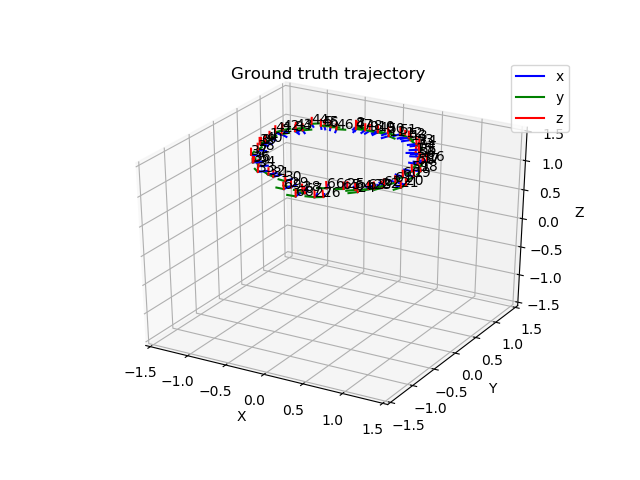
\includegraphics[width=80mm]{../quad/basic-reg-saves/rtrj_gt.png}
  \caption{Ground truth from Vicon}
  \end{subfigure}
  \\
  \begin{subfigure}[t]{0.5\textwidth}
  \centering
    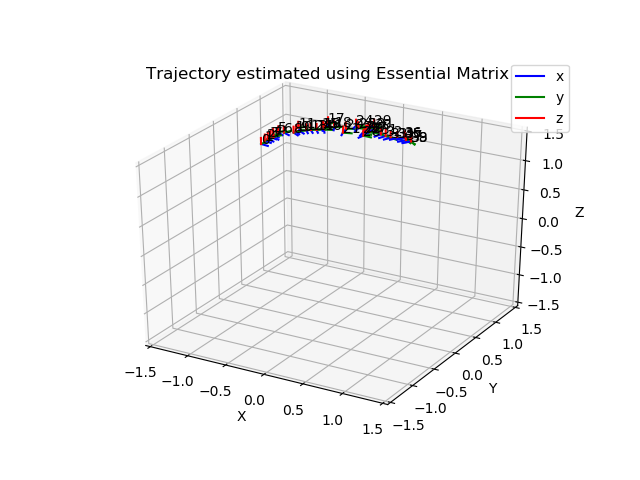
\includegraphics[width=80mm]{../quad/basic-reg-saves/rtrj_rgb.png}
  \caption{Estimated trajectory for Essential Matrix method, start at origin. Note axes scaling x2}
  \end{subfigure}%
  ~
  \begin{subfigure}[t]{0.5\textwidth}
  \centering
    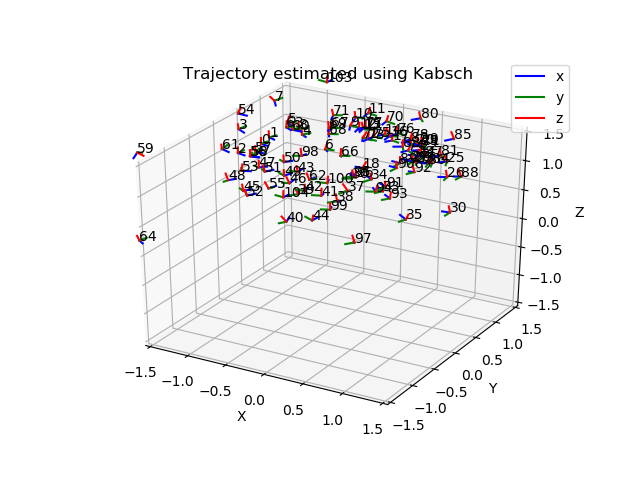
\includegraphics[width=80mm]{../quad/basic-reg-saves/rtrj_d.png}
  \caption{Estimated trajectory for Kabsch method, start at origin}
  \end{subfigure}
  \caption{Trajectory visualizations for second quad dataset}
  \label{f: quad2 trj}
\end{figure}

\begin{figure}[h]
  \centering
  \begin{subfigure}[t]{\textwidth}
  \centering
  \includegraphics[width=120mm]{../quad/matches/1533791935.37_essential.png}
  \caption{Points used for Essential Matrix}
  \end{subfigure}%
  \\
  \begin{subfigure}[t]{\textwidth}
  \centering
  \includegraphics[width=120mm]{../quad/matches/1533791935.37_kabsch.png}
  \caption{Points used for Kabsch}
  \end{subfigure}%
  \caption{Matches after RANSAC (inliers) between two frames}
  \label{f: matches}
\end{figure}


\bibliographystyle{abbrvnat}
\bibliography{../Report/ENGN4217}

\end{document}